\begin{frame}{Summary}
\par An approach that allows agents to reason equitably on the basis of spatial, social and temporal dimensions
\vspace{.4cm}
\par How to offer agents visibility on the temporal dimension as it is already the case for the spatial and social dimension?
\par \alert{$\rightarrow$ The temporal environment} allows the agent to share, store and perceive temporal information
\par \alert{$\rightarrow$ The Agent-Group-Role-Environment-Time (AGRET)} allows the consideration of the 3 dimensions in the same way
\medbreak
\par How to take into account information about the future in the agent's anticipatory reasoning?
\par \alert{$\rightarrow$ The temporal environment} offers agents accessibility on the future dimension of time
\vspace{.4cm}
\end{frame}

\begin{frame}{Summary}
\par \textbf{Multi-agent level}: 
\begin{itemize}
    \item Evolution of multi-agent simulation to  consider the temporal dimension in the same way as the spatial and the social dimension
    \item Optimisation of the agents behaviours choice relevance
\end{itemize} 
\medbreak
\par \textbf{Smart city level}: 
\begin{itemize}
    \item Taking into account the 3 dimensions of the territorial system (space, organization, time)\footnote{ROLLAND-MAY, Christiane. Évaluation des territoires: concepts, modèle, méthodes. Hermès science publications, 2000.}
    \item Generate higher levels of user engagement: exchange and processing of information 
\end{itemize}
\note{
L'intelligence dont il est sujet dans la ville intelligente est notamment une forme d'intelligence participative qui émerge des interactions entre les citoyens et le système.
}
    
\end{frame}

\begin{frame}{Further work}
\par Are there other non-time-constrained environments?
\par \alert{$\rightarrow$ Observation environments for example}
\vspace{1cm}
\par Could social media be exploited to a greater extent?
\par \alert{$\rightarrow$ Define more advanced visibility and accessibility rules}
\begin{itemize}
    \item Networks: circle of friends, social groups, etc.
\item Popularity: reactions, like, etc.
\end{itemize}

\note{
\par Les contributions de cette thèse donnent lieu à plusieurs pistes de recherches. Nous en sélectionnons quelques unes qui nous paraissent particulièrement interessantes.
\par L'introduction du nouveau type d'environnement de nature temporel nous a fait prendre conscience de l'existance d'au moins deux types d'environnements : les environnements contraints par le temps comme l'environnement spatial et l'environnement social. Les environnements non-contraints par le temps comme l'environnement temporel. Nous nous posons alors la question sur la possibilité d'existance d'autres environnements non contraints par le temps, des environnements, des méta-environnement qui évoluent hors du temps. Nous pensons par exemple aux environnements d'observation dont le fonctionnement nous semble sortir du cadrade limité par le temps.
\par Une autre perspective qui nous semble interessante vis à vis du cadre des systèmes multi-agents et d'une manière plus générale, vis-à-vis des smart cities, consiste en l'exploitation des réseaux sociaux.
\par Une utilisation consisterait à définir des règles de visibilité et d'accessibilité en fonction des réseaux sociaux. Nous citons notamment deux notions utilisées dans les réseaux sociaux qui nous semble interessantes:
\begin{item}
\item Les réseaux d'accointances : cercle d'ami, groupe sociaux
\item La notion de popularité : les réactions, le pouce "j'aime" qui permet de qualifier l'importance d'une information.
\end{item}
}
    
\end{frame}

\begin{frame}{Further work}
\begin{figure}
    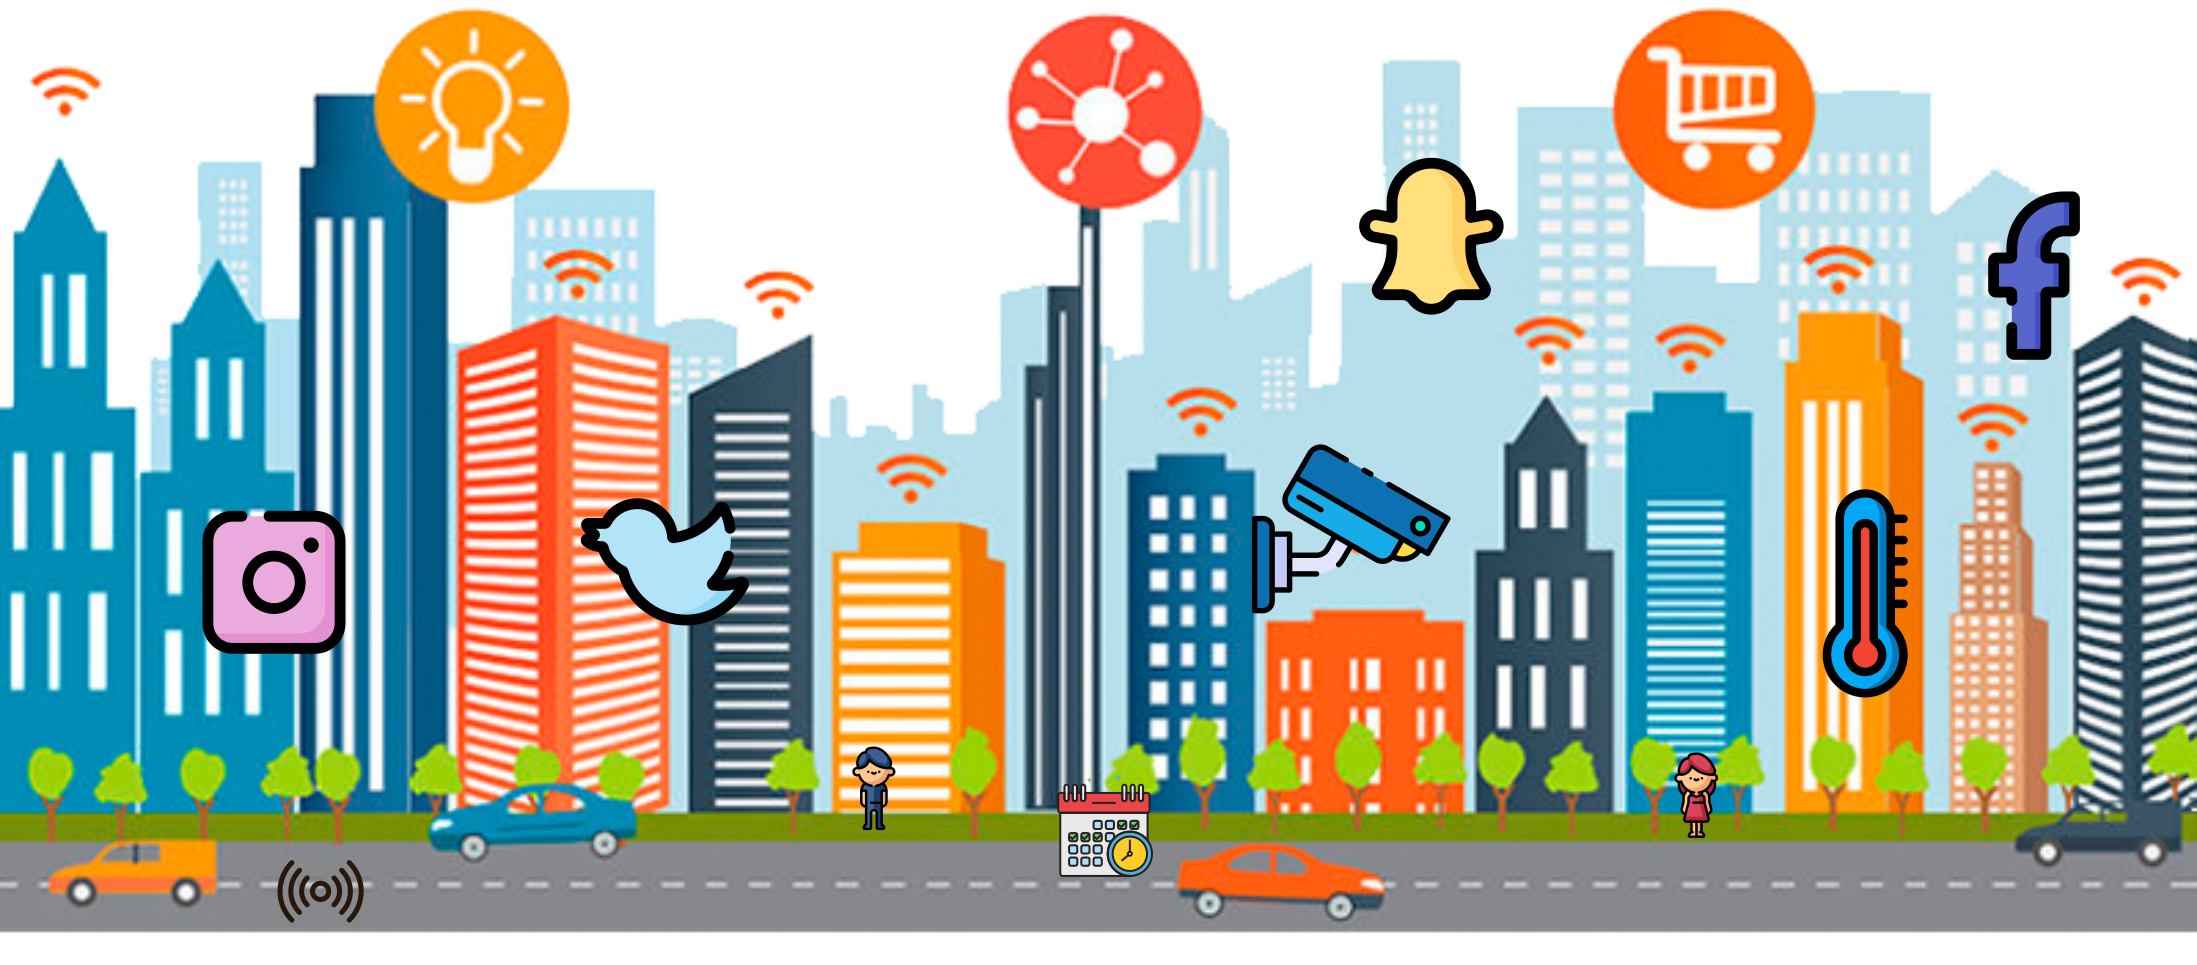
\includegraphics[width=\linewidth]{figures/smartcity.png}
\end{figure}
\centering
Promote the emergence of standards and protocols for smart cities
%reboucler sur les smart cities
\note{Les réseaux sociaux sont notamment très fortement utilisées actuellement dans le villes. Son exploitation devrait nous permettre d'optimiser la participation et l'engagement du citoyen au niveau du système, favorisant encore plus l'émergence des standards et protocoles propres aux villes intelligente}
\end{frame}